\section{Modeling} \label{sec:modeling}

% \begin{figure}
% \begin{minipage}{0.45\textwidth}
% \centering
% \subfloat[\label{fig:classD_rect_sch1} A licking tiger ]{\includegraphics[width=0.7\textwidth]{tiger1.jpg}}\\
% \subfloat[\label{fig:classD_rect_sch2} A mother tiger]{\includegraphics[width=0.7\textwidth]{tiger2.jpg}}
%   \caption{ \label{fig:classD_rect_sch}Adorable tigers}
%   \vspace{-10pt}
% \end{minipage}
% \qquad
% \begin{minipage}{0.45\textwidth}
%     \centering
%     \includegraphics[width=\textwidth]{tiger3.jpg}
%      \caption{ \label{fig:classD_rect_analysis}A smiling tiger}
%      \vspace{-10pt}
% \end{minipage}
% %\vspace{-10pt}
% \end{figure}

The traditional assumption of piece-wise linear inductor current is invalid in practical high-frequency dc-dc converters. Instead, it is more accurate to model the measured inductor current as a ramp added by an interference function.
We illustrate a new model of interfered inner current loop. We found that the reasons of long-time settling and instability in the practical converter can be effectively explained by this model. We first define the interference function as following: 
\begin{definition}
$f(t)$, the interference function in continuous time satisfies the following properties \begin{enumerate*} [label=(\roman*)]  \item $f(t)$ is cycle-invariant; \item $f(t)$ has a bounded amplitude of $[0, A_{\text{max}}]$ and a bounded frequency spectrum of $[\omega_{\text{min}}, \omega_{\text{max}}]$.
\end{enumerate*} 
\end{definition}

\begin{figure}
\begin{minipage}{0.32\textwidth}
    \centering
    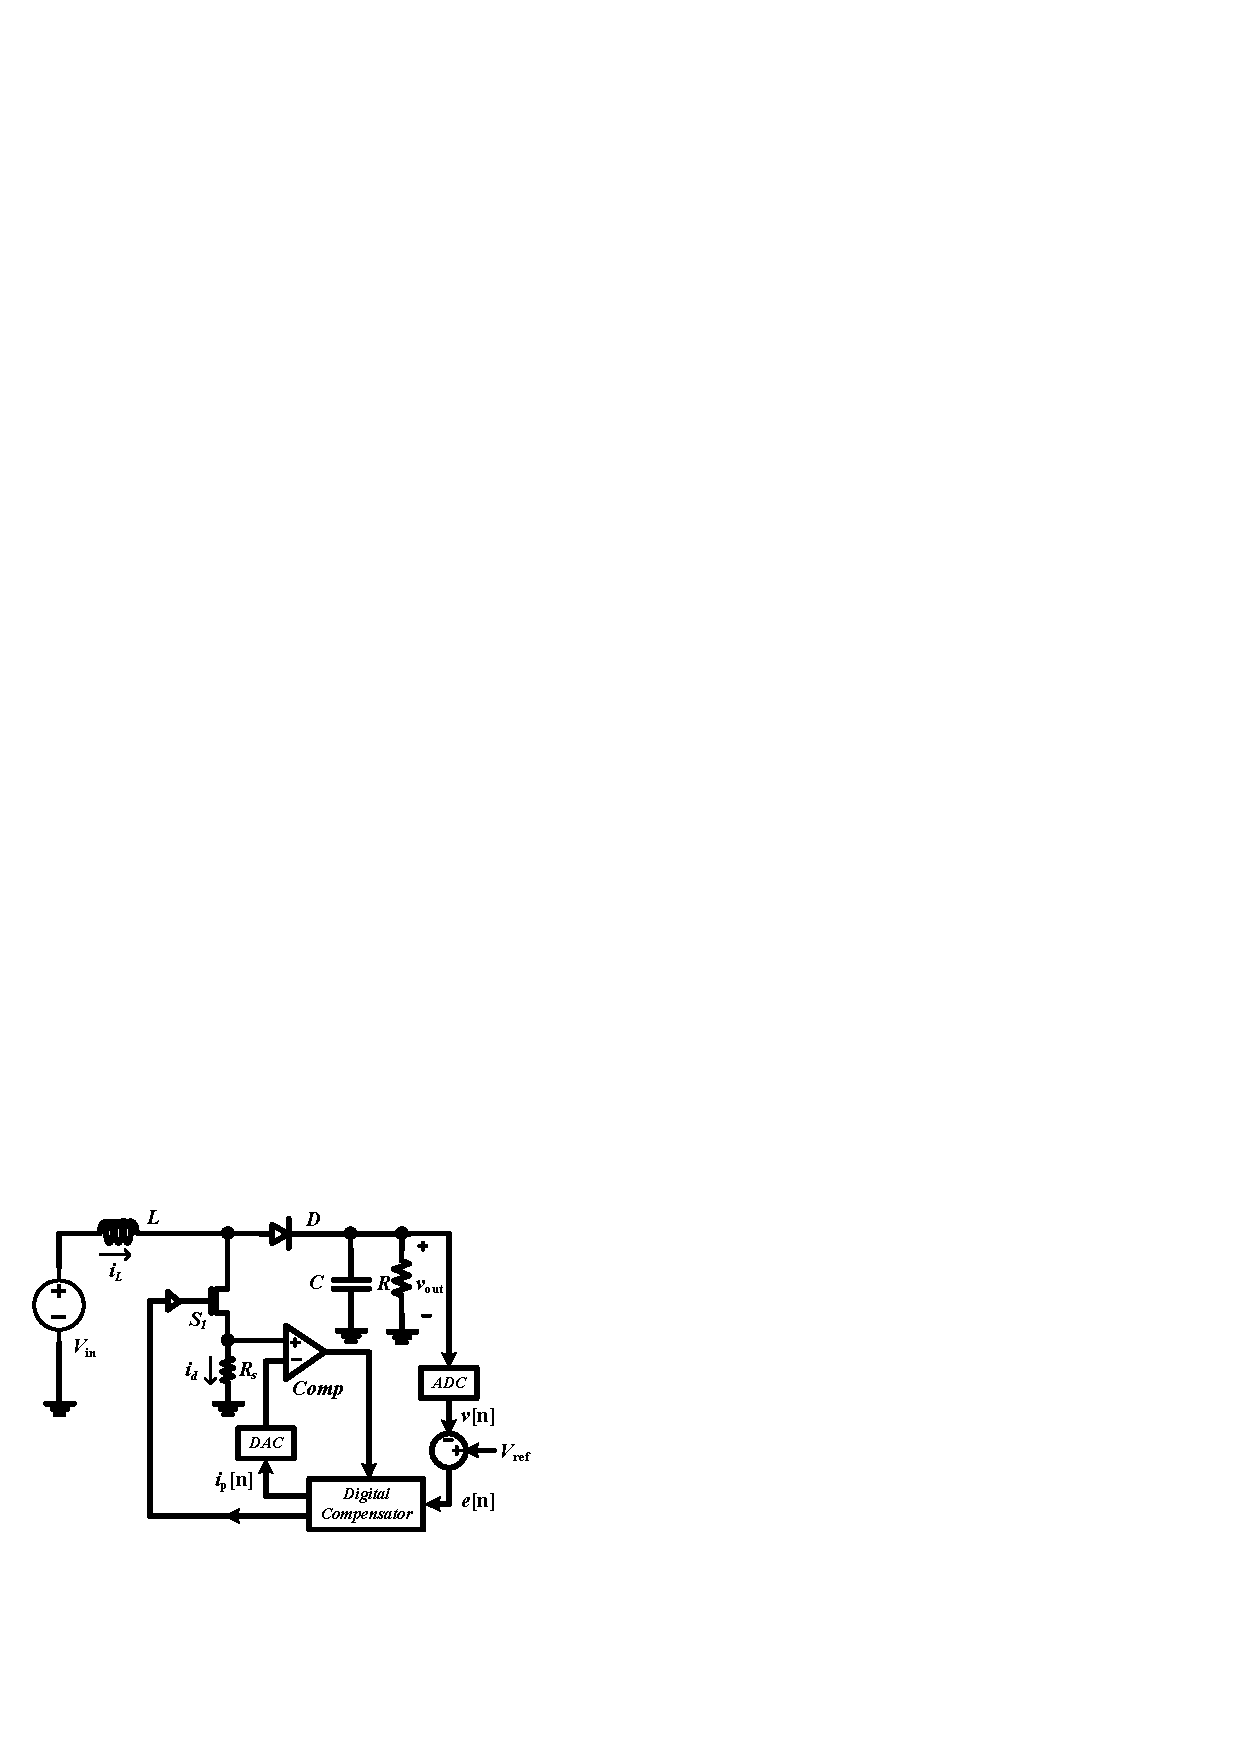
\includegraphics[width=\textwidth]{Figure/section2/schematiceboost.pdf}
    \caption{ \label{fig:eboostschmatic} Schematic diagram of a digitally-controlled CM-COT boost converter.}
\end{minipage}
~
\begin{minipage}{0.32\textwidth}
    \centering
    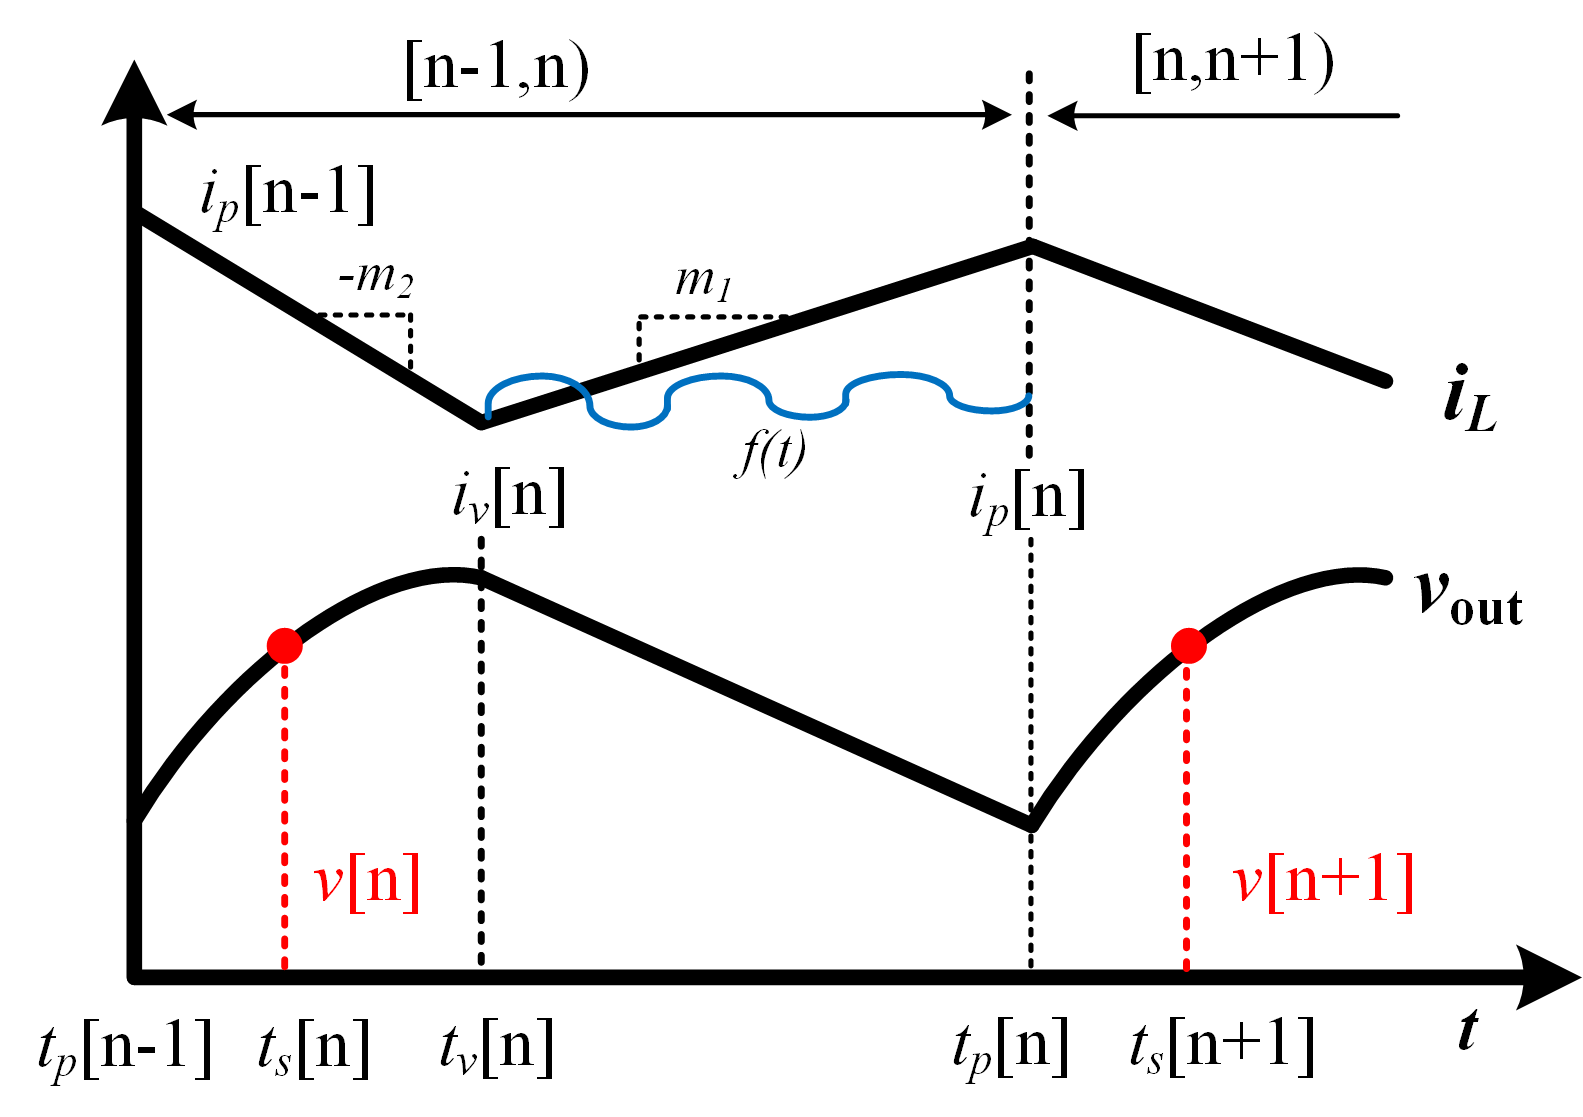
\includegraphics[width=\textwidth]{Figure/section2/eboostwaveform.png}
  \caption{\label{fig:lcwavefrom} Inductor current and capacitor voltage waveforms of a digitally-controlled CM-COT boost converter.}
\end{minipage}
~
\begin{minipage}{0.32\textwidth}
    \centering
    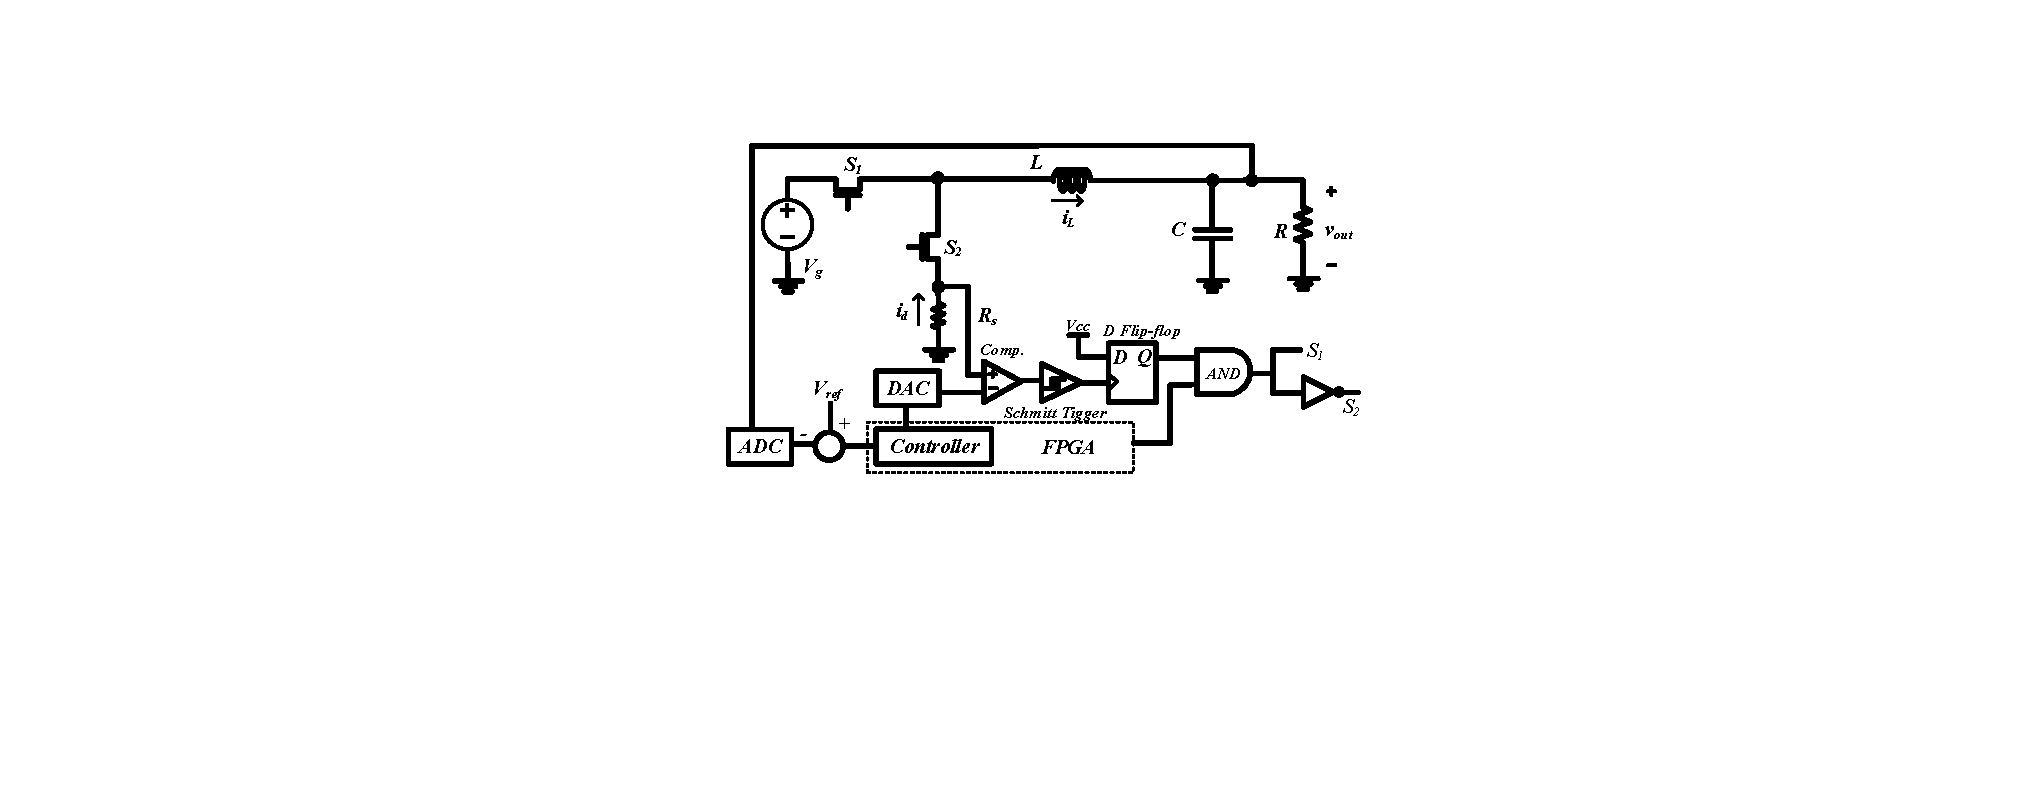
\includegraphics[width=\textwidth]{Figure/section2/currentdetection.pdf}
    \caption{\label{fig:currentdection} Analog valley-current controller for constant-on-time
    current-mode buck.}
\end{minipage}
\end{figure}

The example converter plant we used is a current-mode boost converters using constant off-time (CM-COT boost converter) as shown in Fig.\;\ref{fig:eboostschmatic}.
$i_c[n]$ is the current command from the outer loop every cycle. Our model of the interfered inner current loop can by described by following difference equations:
\begin{align} \label{sys:innerloop}
i_p[n] &= i_p[n-1] - m_2t_{\text{off}} +m_1t_{\text{on}}[n], \\
i_c [n] &= i_p[n] +f(t_{\text{on}}[n]).
\end{align}
The $I_e$ and $T_{\text{on}}$ at equilibrium can be obtained by letting $i_p[n+1] = i_p[n]$, $t_{\text{on}}[n+1] = t_{\text{on}}[n]$. $I_e$ and $I_c$’s relationship are govern by an implicit function $g(I_e, I_c) = 0$. We define an explicit mapping $\mathcal{T}: \mathcal{R}_+ \rightarrow \mathcal{R}_+$ from the inductor current command $I_c$ to the actual inductor current $I_e$ in steady state.

Although no assumptions mathematically guarantees that mapping $\mathcal{T}$ is a single-valued and monotonically non-decreasing explicit function. However, our special design using first-event-triggering mechanism guarantees these properties.
As shown in Fig\;\ref{fig:multieventtrigger}, the possibile triggering time instants can be $t_1$, $t_2$,$t_3$ or $t_4$. The D flip-flop in Fig\;\ref{fig:currentdection} always latch the first comparator detection, which is then reset by the FPGA at the next switching cycle. This design guarantee $t_1$ to be the triggering time instant. A generic function $\mathcal{T}$ is like the shape in Fig\;\ref{fig:functionT}. 
One defect of the function $\mathcal{T}$ is that it might includes jump discontinuity points. For $I_e \in [I_{f_1}-I_{f_2}]$ or $I_{f_3}-I_{f_4}$, there is no correct peak current command $I_c$ which can position the real pwak current.
\begin{definition}
we define the \emph{unreachable equilibrium set} $U\!E \triangleq [I_{f_1},I_{f_2}] \cup [I_{f_3},I_{f_4}],\ldots$. Lebesgue measure of the $U\!E$ is $\lambda(U\!E)$.
\end{definition}
We do not recommend having $\lambda(U\!E) \neq 0$ for control practice because the inner current loop will not be able to position the current to wherever the outer loop controller wants. We give the following theorem without proof to show the relationship between $\lambda(U\!E)$ and interference function $f(t)$.
\begin{theorem} \label{th:equexcond}
$\mathcal{T}$ is an onto-function if and only if the measured inductor current waveform $m_1t+f(t)$ is strictly monotonic.
\end{theorem}
\subsection{Stability}
Under the condition of Theorem \ref{th:equexcond}, we would like to study the stability of the equilibrium. Suppose the equilibrium is at $i_p[n] = I_e$, $t_{\text{on}}[n]= T_{\text{on}}$, $i_c[n] = I_c$, 
We translate the equilibrium to the origin by defining $\tilde i_p[n] = i_{p}[n] - I_{e}$, $ \tilde t_{\text{on}}[n] = t_{\text{on}}[n] -  T_{\text{on}}, \tilde i_c[n] = i_c[n] - I_c$. 
\begin{align}  \label{ID1}
\tilde i_p[n] &= \tilde i_p[n-1] +  m_1 \tilde t_{\text{on}}[n] \\
\tilde i_c [n] &= \tilde i_p[n] +f(t_{\text{on}}[n]) - f(T_{\text{on}}).
\end{align}
We assume the peak current command $ i_c[n]$ from outer voltage loop is fixed at $I_{c}$. 
% We also assume that the the interference function $f$ is strictly monotonic and odd within the domain of our interests, so that the $f^{-1}$ exists and is an odd function as well,
% \begin{align}
% \tilde i_p[n] &= \tilde i_p[n-1] - m_1 (-\tilde t_{\text{on}}[n]), \\
% - \tilde  t_{\text{on}}[n]  &= f^{-1} (\tilde  i_p[n] - f(T_{on})).
% \end{align}

The resulting system can be formulated into a Lure system as shown in Fig\;\ref{fig:luresystem}. By applying the circle criterion, we prove the following theorem to show the stability conditions for the system (\ref{sys:innerloop}) under any disturbance:
\begin{theorem} \label{th:gloasystab}
The $A_{\text{max}} \omega_{\text{max}} < (m_1/2) $ if and only if the inner current loop is \emph{globally asymptotically stable}.
\end{theorem}
\begin{proof}

\end{proof}

\subsection{Performance}
In system (\ref{sys:innerloop}), we view the current command sequence $\tilde i_c [n]$ as the input and the peak inductor current sequence $\tilde i_p [n]$ as the output. Ideally, the peak inductor current is assumed to follow the peak-current command with small overshoot and fast speed. However, with interference amplitude increasing, one could expect the convergence speed gradually slow down and overshoot gradually increases. 
 
We show a $Z$-transform method to systematically analyze the performance of system (\ref{sys:innerloop}) including settling time, overshoot and stability margin. 

We linearize the system (\ref{sys:innerloop}) and have
\begin{align} \label{sys:linear}
    \tilde i_p[n] &= \tilde i_p[n-1] +  m_1 \tilde t_{\text{on}}[n], \\
    \tilde i_c [n]  & = \tilde i_p[n-1] + (f^{'}(T_{\text{on}}) + m_1)\tilde t_{\text{on}} [n].
\end{align}
 We define an equivalent local slope $s_0 = f^{'}(T_{\text{on}}) + m_1$, slope ratio $\beta = m_1/s_0$, and pole of inner current loop $a = 1-\beta$. Then system (\ref{sys:innerloop}) can be simplified as 
\begin{align}
\tilde i_p[n] &=  \beta \tilde i_c [n] + a \tilde i_p[n-1].
\end{align}
Note that although the discretized data does not have a uniform corresponding to physical time domain, $Z$-transform can still be applied \cite{Cui2018a},
\begin{align}
    C_2(z) = \frac{\beta}{1- a z^{-1}}.
\end{align}
Ideally, $\beta = 1$, $a = 0$ and the pole of $C_2(z)$ locates at 0, meaning $C_2(z)$ is deadbeat. 
The larger the $|a|$ is, the longer transient under reference step the inner loop will have.

Because of the uncertainty of the derivative of f, While the operating points is moving, the pole $a$ is within the range
%  $ [1 - m_1/(m_1 + m_s + f^{'}_{\text{min}}), 1-m_1/(m_1 + m_s + f^{'}_{\text{max}})]$. 
\begin{align}
a_{\text{min}} &= 1 - \frac{m_1}{(m_1 + m_s + f^{'}_{\text{min}})} \le a \le   a_{\text{max}} = 1 - \frac{m_1}{(m_1 + m_s + f^{'}_{\text{max}})}.
\end{align}

By denoting $a \in [a_{\text{min}}, a_{\text{max}}]$, 
we can analyze the Worst case settling cycles $-log^{-1}(a)$ and Worst case overshoot (ref) and stability margin $\text{max} \{1+a_{\text{min}}, 1-a_{\text{max}}\}$.

Although the performance analysis is in the discrete time ($5S$), the settling time and overshoot in time domain is predictable by settling cycle and overshoot by theorem 2 and 3 \cite{Cui2018a}.


\begin{figure}
\begin{minipage}{0.32\textwidth}
    \centering
    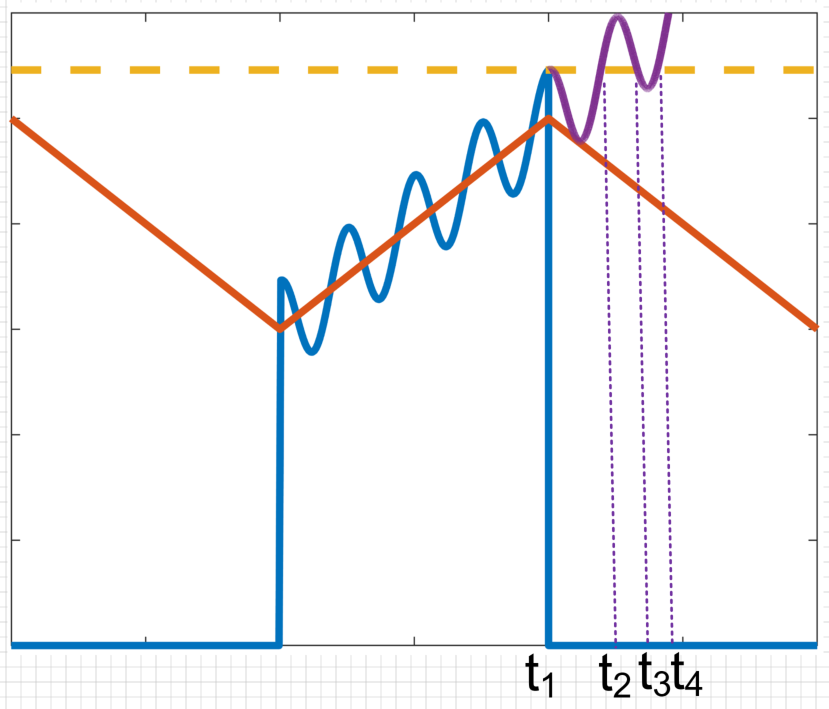
\includegraphics[width=\textwidth]{Figure/section2/Multievent_trigger.png}
    \caption{ \label{fig:multieventtrigger} First-event trigger using D flip-flop.}
\end{minipage}
~
\begin{minipage}{0.32\textwidth}
    \centering
    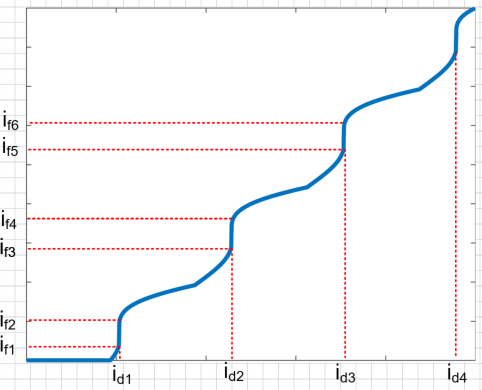
\includegraphics[width=\textwidth]{Figure/section2/functionT.png}
  \caption{  \label{fig:functionT} A common graph for the function $T$.}
\end{minipage}
~
\begin{minipage}{0.32\textwidth}
    \centering
    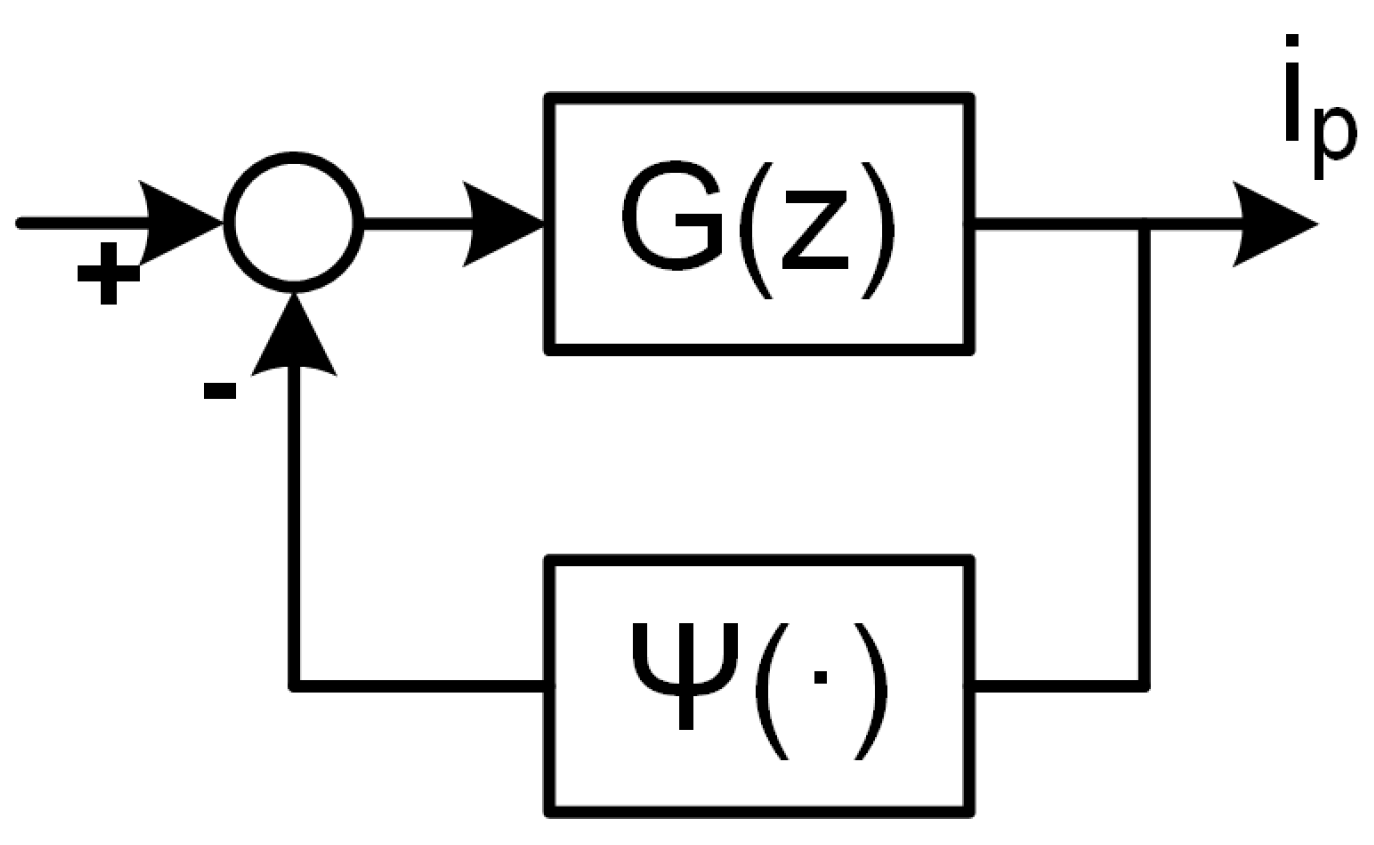
\includegraphics[width=\textwidth]{Figure/section2/luresystem.PNG}
    \caption{\label{fig:luresystem} Lure system representation of the inner current loop.}
\end{minipage}
\end{figure}


A geometric explanation of the current command block dynamics by assuming the noise is a slow varying signal and can be considered as a ramp error


The stability criterion of the current-mode buck converter using constant on-time and current-mode boost converter using constant on-time is given as follows:


\begin{figure}
\begin{minipage}{0.32\textwidth}
    \centering
    \includegraphics[width=\textwidth]{Figure/catsatind3.pdf}
    \caption{ \label{catonsatind} First-event trigger using D flip-flop.}
\end{minipage}
~
\begin{minipage}{0.32\textwidth}
    \centering
    \includegraphics[width=\textwidth]{Figure/ebuckschematicrenew.pdf}
  \caption{  \label{circuitdiagram} A common graph for the function $T$.}
\end{minipage}
~
\begin{minipage}{0.32\textwidth}
    \centering
    \includegraphics[width=\textwidth]{Figure/waveform2.pdf}
    \caption{\label{eboostderivation} Inductor current and capacitor voltage waveforms of a CM-COT buck converter with saturaing inductor.}
\end{minipage}
\end{figure}



% \begin{figure}
% \begin{minipage}{0.49\textwidth}
% \subfloat[\label{fig:licking_tiger}A licking tiger]{\includegraphics[width=0.45\textwidth]{figures/tiger1.jpg}} \quad
% \subfloat[\label{fig:mother_tiger}A mother tiger]{\includegraphics[width=0.45\textwidth]{figures/tiger2.jpg}}
% \caption{\label{fig:beautiful_tiger}Beautiful tigers}
% \end{minipage}
% %%\hfill
% \begin{minipage}{0.49\textwidth}
% \subfloat[\label{fig:smiling_tiger}A smiling tiger]{\includegraphics[width=0.45\textwidth]{figures/tiger3.jpg}} \quad
% \subfloat[\label{fig:phd_tiger}A Ph.D. tiger]{\includegraphics[width=0.45\textwidth]{figures/tiger4.jpg}}
% \caption{ \label{fig:more_beautiful_tiger}More beautiful tigers. Everyone loves tigers.}
% \end{minipage}
% \end{figure}



% \begin{wrapfigure}{r}{0.33\textwidth}
%   \vspace{-20pt}
%   \begin{center}
%     \includegraphics[width=0.32\textwidth]{tiger3.jpg}
%   \caption{ \label{fig:Zrect_eq_model}A smiling tiger}
%   \end{center}
%   \vspace{-20pt}
% \end{wrapfigure}
